\documentclass[12pt,addpoints,answers]{exam}
\usepackage[margin=1in]{geometry}
\usepackage{amsmath,amssymb,amsfonts}
\usepackage{graphicx}
\usepackage{multirow}
\usepackage[T1]{fontenc}
\usepackage[utf8]{inputenc}
\printanswers
\unframedsolutions
\renewcommand{\solutiontitle}{}

\begin{document}
\section*{Pre-Calculus 40S --- January 2013}

\begin{questions}

\question
\leavevmode
% Q1 | Pre-Calculus 40S --- January 2013
Gina correctly started to answer the following question. Complete her solution.\\
Question: Solve the following equation for all real values of $\theta$.\\
Express your answer in radians correct to 3 decimal places.

$$
3 \sin ^{2} \theta-14 \sin \theta-5=0
$$

Gina's solution: $3 \sin ^{2} \theta-14 \sin \theta-5=0$

$$
(3 \sin \theta+1)(\sin \theta-5)=0
$$
\begin{solution}
\textbf{Solution:}\par

\textbf{Method 1}\par
$$
\begin{array}{r}
3 \sin ^{2} \theta-14 \sin \theta-5=0 \\
(3 \sin \theta+1)(\sin \theta-5)=0
\end{array}
$$

$$
\begin{array}{lll}
\sin \theta=-\frac{1}{3} & \sin \theta=5 & 1 / 2 \text { mark for } \sin \theta=5 \\
\text { no solution } & 1 / 2 \text { mark for no solution }
\end{array}
$$

$$
\theta_{r}=0.339837
$$

$$
\theta=3.481429,5.943348 \quad 1 \text { mark }\left(\frac{1}{2} \text { mark for each value of } \theta\right)
$$

$$
\begin{aligned}
& \theta=3.481+2 k \pi, k \in \mathrm{I} \\
& \theta=5.943+2 k \pi, k \in \mathrm{I}
\end{aligned}
$$

1 mark for general solution

Note(s):

\begin{itemize}
  \item give maximum of 2 marks for solution in degrees: $\theta=199.471^{\circ}+360^{\circ} k, k \in \mathrm{I}$
\end{itemize}

$$
\theta=340.529^{\circ}+360^{\circ} k, k \in \mathrm{I}
$$


\textbf{Method 2}\par
$$
y=3 \sin ^{2} \theta-14 \sin \theta-5
$$

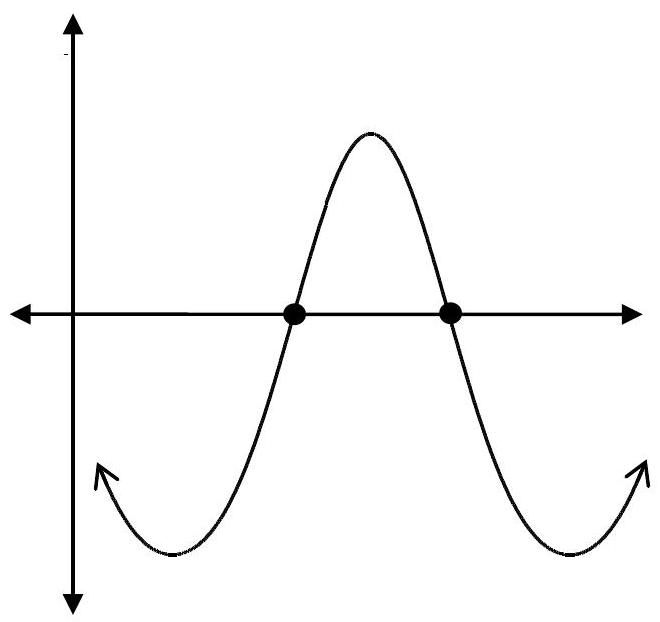
\includegraphics[width=0.6\linewidth]{figures/2795df6c-6e2d-4017-aae1-564aebe344d4-02_622_660_603_207}\\
or\\
Find all zeros over the reals.

$$
\theta=3.481+2 k \pi, k \in \mathrm{I}
$$

$\theta=5.943+2 k \pi, k \in \mathrm{I}$

$$
\frac{1}{2} \text { mark for equation }
$$

$\frac{1}{2}$ mark for justification

1 mark for general solution\\
3 marks
\end{solution}

\question
\leavevmode
% Q2 | Pre-Calculus 40S --- January 2013
Find and simplify the 6 th term in the binomial expansion of $\left(3 x^{4}-\frac{1}{x^{3}}\right)^{9}$.
\begin{solution}
\textbf{Solution:}\par
$$
\begin{array}{rlr}
t_{6} & ={ }_{9} C_{5}\left(3 x^{4}\right)^{4}\left(-\frac{1}{x^{3}}\right)^{5} & 2 \text { marks (1 mark for }{ }_{9} C_{5}, 1 / 2 \text { mark for each consistent factor) } \\
& =(126)\left(81 x^{16}\right)\left(-\frac{1}{x^{15}}\right) & \\
& =-10206 x & \begin{array}{l}
1 \text { mark for simplification }(1 / 2 \text { mark for evaluating coefficient, } 1 / 2 \text { mark } \\
\text { for simplifying variable })
\end{array}
\end{array}
$$
\end{solution}

\question
\leavevmode
% Q3 | Pre-Calculus 40S --- January 2013
The number of times a website is visited can be modeled by the function:

$$
A=800(e)^{r t}
$$

where $A=$ the total number of visitors at time $t$\\
$t=$ the time in days $(t \geq 0)$\\
$r=$ the rate of growth\\
After 5 days, 40000 people have visited the site.\\
Determine the number of visitors expected after 9 days.\\
Express your answer as a whole number.
\begin{solution}
\textbf{Solution:}\par

\textbf{Method 1}\par
$40000=800 e^{r 5}$\\
$\frac{1}{2}$ mark for substitution

$$
\begin{array}{rlr}
\frac{40000}{800} & =e^{5 r} & \\
\ln 50 & =\ln e^{5 r} & 1 / 2 \text { mark for applying logs } \\
\ln 50 & =5 r & 1 \text { mark for log theorem } \\
\frac{\ln 50}{5} & =r & \\
r & =0.782404601 &
\end{array}
$$

$$
\begin{aligned}
& A=800 e^{(0.782404601)(9)} \\
& A=914610.103 \\
& A=914610
\end{aligned}
$$

$\frac{1}{2}$ mark for substitution\\
$\frac{1}{2}$ mark for calculations with base $e$\\
3 marks


\textbf{Method 2}\par
Use calculator to find the value of $r$.\\
$y=40000$\\
$y=800 e^{5 x}$\\
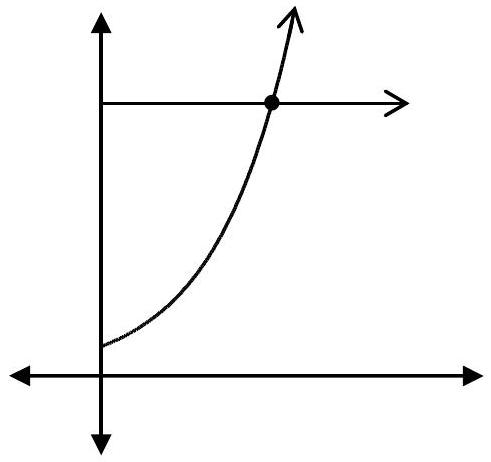
\includegraphics[width=0.6\linewidth]{figures/2795df6c-6e2d-4017-aae1-564aebe344d4-05_462_491_898_191}\\
or\\
Find the point of intersection of these two functions.

$$
x=0.782404601
$$

Substitute $x$ for $r$ into formula.

$$
\begin{aligned}
\therefore A & =800 e^{(0.782404601)(9)} \\
A & =914610.103 \\
A & =914610
\end{aligned}
$$

$\frac{1}{2}$ mark for equations\\
$\frac{1}{2}$ mark for justification

1 mark for finding the value of $x$ at the intersection point

1 mark for value of $A$

3 marks
\end{solution}

\question
\leavevmode
% Q4 | Pre-Calculus 40S --- January 2013
Solve algebraically:

$$
10^{3 x}=7^{x+5}
$$

Express your answer correct to 3 decimal places.
\begin{solution}
\textbf{Solution:}\par

\textbf{Method 1}\par
$$
\begin{array}{rlrl}
10^{3 x} & =7^{x+5} & \\
\log 10^{3 x} & =\log 7^{x+5} & 1 / 2 \text { mark for applying logs } \\
3 x(\log 10) & =(x+5) \log 7 & 1 \text { mark for power rule } & \\
3 x \log 10 & =x \log 7+5 \log 7 & & \\
3 x \log 10-x \log 7 & =5 \log 7 & 1 / 2 \text { mark for collecting terms with } x & \\
x & =\frac{5 \log 7}{3 \log 10-\log 7} & 1 / 2 \text { mark for solving for } x \\
x & =1.960873 & 1 / 2 \text { mark for evaluating quotient of } \\
x & =1.961 & & \text { logarithms }
\end{array}
$$


\textbf{Method 2}\par
$$
\begin{aligned}
10^{3 x} & =7^{x+5} \\
\log 10^{3 x} & =\log 7^{x+5} \\
3 x(\log 10) & =(x+5) \log 7 \\
3 x & =x \log 7+5 \log 7
\end{aligned}
$$

$3 x-x \log 7=5 \log 7$

$$
\begin{aligned}
& x=\frac{5 \log 7}{3-\log 7} \\
& x=1.960873 \\
& x=1.961
\end{aligned}
$$
\end{solution}

\question
\leavevmode
% Q5 | Pre-Calculus 40S --- January 2013
A word contains two Ms, two Es, two Ns, and no other repeated letters.\\
Suppose one of the Ns is replaced by an M.\\
Will this replacement result in greater or fewer permutations?\\
Justify your reasoning.
\begin{solution}
\textbf{Solution:}\par

\textbf{Method 1}\par
$2 \mathrm{Ms}, 2 \mathrm{Es}, 2 \mathrm{Ns}: \frac{(\text { total number of letters })!}{2!2!2!}$ 1 mark for dividing the total number of letters by $2!2!2!$

$$
\frac{(\text { total number of letters })!}{8}
$$

$3 \mathrm{Ms}, 2 \mathrm{Es}, 1 \mathrm{~N}$ : $\frac{\text { (total number of letters)! }}{3!2!1!}$ 1 mark for dividing the total number of letters by $3!2!1!$

$$
\frac{(\text { total number of letters })!}{12}
$$

If one of the Ns is changed to an M, there would be fewer permutations.


\textbf{Method 2}\par
If one of the Ns is changed to an M, there would be fewer permutations because you would be dividing the total number of letters by a larger number.

2 marks for justification\\
2 marks
\end{solution}

\question
\leavevmode
% Q6 | Pre-Calculus 40S --- January 2013
There is a group of 16 boys and 12 girls. How many ways can a committee of 3 people be formed if there must be at least 2 girls on the committee?\\
Express your answer as a whole number.
\begin{solution}
\textbf{Solution:}\par

\textbf{Method 1}\par
Case 1: 2 girls, 1 boy\\
Case 2: 3 girls

$$
{ }_{12} C_{2} \cdot{ }_{16} C_{1}=1056
$$

$$
{ }_{12} C_{3}=220
$$

$$
1056+220=1276
$$

1 mark for case 1 ( $\frac{1}{2}$ mark for each factor shown in a product)\\
1 mark for case 2\\
1 mark for addition of cases\\
3 marks


\textbf{Method 2}\par
Case 1: 2 boys, 1 girl\\
Case 2: 3 boys\\
All possibilities\\
${ }_{16} C_{2} \cdot{ }_{12} C_{1}=1440$

$$
{ }_{16} C_{3}=560
$$

${ }_{28} C_{3}=3276$\\
$3276-1440-560=1276$

1 mark for case 1 ( $\frac{1}{2}$ mark for each factor shown in a product)\\
1 mark for case 2\\
$\frac{1}{2}$ mark for all possible cases\\
$\frac{1}{2}$ mark for subtraction from total\\
3 marks
\end{solution}

\question
\leavevmode
% Q7 | Pre-Calculus 40S --- January 2013
A student is using the formula $s=\theta r$ to find an arc length of a circle. Given a central angle measure of $35^{\circ}$ and a radius of 6 cm , the student's solution is as follows:

$$
\begin{aligned}
& s=(35)(6) \\
& s=210 \mathrm{~cm}
\end{aligned}
$$

Explain why this solution is incorrect.\\
Write the correct solution.
\begin{solution}
\textbf{Solution:}\par
When using the formula $s=\theta r$, the angle must be in radians. $\frac{1}{2}$ mark for explanation\\
$35^{\circ}\left(\frac{\pi}{180^{\circ}}\right)=\frac{35 \pi}{180} \quad$ or $\quad \frac{7 \pi}{36}$\\
$\therefore s=\theta r$

$$
\begin{aligned}
& =\frac{7 \pi}{36}(6) \\
& =\frac{42 \pi}{36} \mathrm{~cm} \quad \text { or } \quad \frac{7 \pi}{6} \mathrm{~cm} \quad \text { or } \quad 3.665 \mathrm{~cm}
\end{aligned}
$$

1 mark for conversion to radians

$$
\frac{1}{2} \text { mark for simplification }
$$

2 marks

Note(s):

\begin{itemize}
  \item award 1 mark for correct final answer with no work
\end{itemize}
\end{solution}

\question
\leavevmode
% Q8 | Pre-Calculus 40S --- January 2013
Given the graph of $f(x)$ below, explain how you would sketch the graph of $y=|f(x)|$.\\
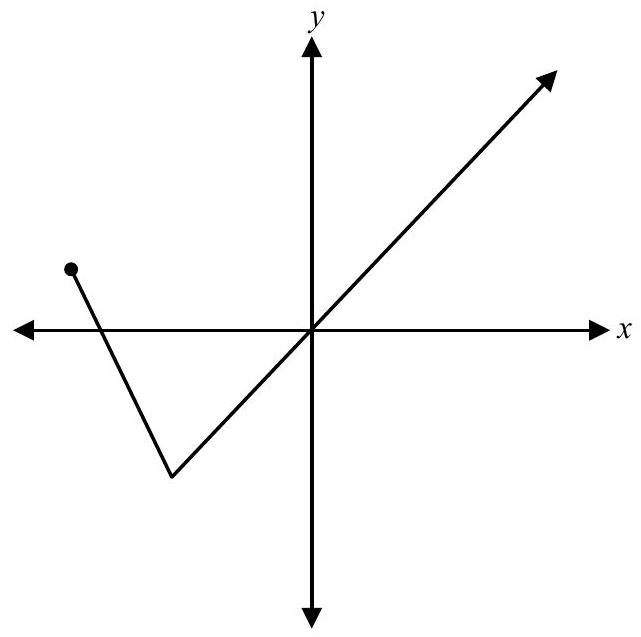
\includegraphics[width=0.6\linewidth]{figures/2795df6c-6e2d-4017-aae1-564aebe344d4-10_637_641_476_249}
\begin{solution}
\textbf{Solution:}\par
The negative $y$ values are reflected over the $x$-axis.

1 mark for explanation\\
1 mark
\end{solution}

\question
\leavevmode
% Q9 | Pre-Calculus 40S --- January 2013
Claire correctly solves the following equation:

$$
\log _{2}(6-x)+\log _{2}(3-x)=2
$$

She finds two possible values of $x$ : $x=2$ and $x=7$.\\
Identify which one of these values is unacceptable and explain why.
\begin{solution}
\textbf{Solution:}\par
If $x$ is greater than 3 , you have a negative argument $\therefore x=2$ but $x \neq 7$.\\
or\\
The domain is restricted to values of $x<3 \therefore x=2$.

1 mark for explanation\\
1 mark
\end{solution}

\question
\leavevmode
% Q10 | Pre-Calculus 40S --- January 2013
Given the graph of the function $f(x)$ below, state the domain of $y=\sqrt{f(x)}$.\\
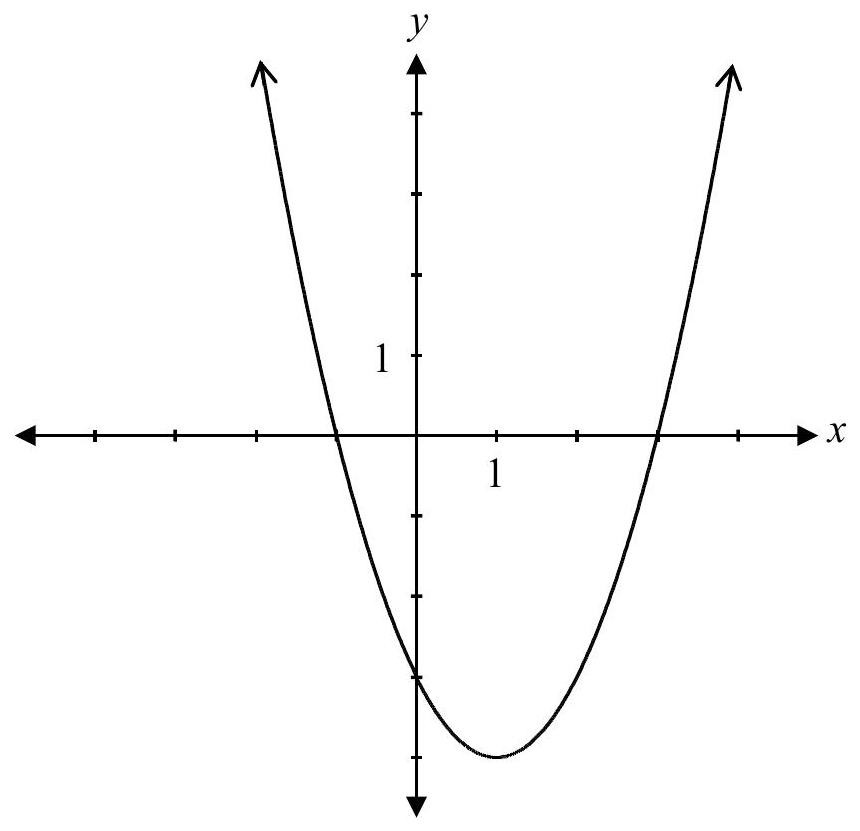
\includegraphics[width=0.6\linewidth]{figures/2795df6c-6e2d-4017-aae1-564aebe344d4-12_831_860_517_234}
\begin{solution}
\textbf{Solution:}\par
The domain is $\{x \in \mathbb{R} \mid x \leq-1$ or $x \geq 3\}$.\\
or

1 mark for domain\\
1 mark
\end{solution}

\question
\leavevmode
% Q11 | Pre-Calculus 40S --- January 2013
The domain is $(-\infty,-1] \cup[3, \infty)$.

A school offers 4 different Science courses, 3 different Mathematics courses, and 2 different English courses.

Julie must select 1 Science course, 1 Mathematics course, and 1 English course. She thinks this creates 9 options for her timetable.

Show why Julie is incorrect.
\begin{solution}
\textbf{Solution:}\par
Julie should have multiplied the number of options.\\
or\\
$4 \times 3 \times 2=24$ different options

1 mark for justification\\
1 mark
\end{solution}

\question
\leavevmode
% Q12 | Pre-Calculus 40S --- January 2013
Explain how Pascal's triangle can be used to determine the coefficients in the binomial expansion of $(x+y)^{n}$.
\begin{solution}
\textbf{Solution:}\par
The $(n+1)^{\text {st }}$ row of Pascal's triangle corresponds to the coefficients of the terms in the expansion of the binomial $(x+y)^{n}$.

1 mark for explanation\\
1 mark
\end{solution}

\question
\leavevmode
% Q13 | Pre-Calculus 40S --- January 2013
Prove the identity below for all permissible values of $x$ :

$$
\frac{1+\cos 2 x}{\sin 2 x}=\cot x
$$
\begin{solution}
\textbf{Solution:}\par

\textbf{Method 1}\par
$$
\begin{aligned}
\text { LHS } & =\frac{1+2 \cos ^{2} x-1}{2 \sin x \cos x} \\
& =\frac{2 \cos ^{2} x}{2 \sin x \cos x} \\
& =\frac{\cos x}{\sin x} \\
& =\cot x \\
& =\text { RHS }
\end{aligned}
$$

1 mark for identity\\
$\frac{1}{2}$ mark for identity\\
1 mark for simplification\\
$\frac{1}{2}$ mark for identity\\
3 marks


\textbf{Method 2}\par
$$
\begin{array}{rlr}
\text { LHS } & =\frac{1+1-2 \sin ^{2} x}{2 \sin x \cos x} & \\
& =\frac{1 / 2 \text { mark for identity }}{2 \sin x \cos x} & \\
& =\frac{1-\sin ^{2} x}{\sin x \cos x} & \\
& =\frac{\cos ^{2} x}{\sin x \cos x} & \\
& =\frac{\cos x}{\sin x} \text { mark for simplification } \\
& =\cot x & \\
& =\text { RHS } & 1 / 2 \text { mark for identity } \\
& 1 / 2 \text { mark for simplification } \\
& \mathbf{3} \text { marks for identity }
\end{array}
$$


\textbf{Method 3}\par
$$
\begin{aligned}
\text { LHS } & =\frac{1+\cos ^{2} x-\sin ^{2} x}{2 \sin x \cos x} \\
& =\frac{2 \cos ^{2} x}{2 \sin x \cos x} \\
& =\frac{\cos x}{\sin x} \\
& =\cot x \\
& =\text { RHS }
\end{aligned}
$$

$\frac{1}{2}$ mark for identity\\
$\frac{1}{2}$ mark for identity\\
$\frac{1}{2}$ mark for identity $\left(1-\sin ^{2} x=\cos ^{2} x\right)$\\
1 mark for simplification\\
$\frac{1}{2}$ mark for identity\\
3 marks
\end{solution}

\question
\leavevmode
% Q14 | Pre-Calculus 40S --- January 2013
Your classmate, Leo, was absent for one of his math lessons.\\
Explain to Leo how to determine the cosecant ratio for an angle in standard position given that $\mathrm{P}(-3,-4)$ is a point on the terminal arm of the angle.
\begin{solution}
\textbf{Solution:}\par

\textbf{Method 1}\par
\begin{itemize}
  \item Locate the point $(-3,-4)$ on the coordinate plane.
  \item Draw a right-angle triangle by connecting the point $(-3,-4)$ to the $x$-axis and to the origin.
  \item The angle created with the $x$-axis and the line connecting the point with the origin (the terminal arm) is $\theta$.
  \item Determine the length of the terminal arm by using the Pythagorean Theorem.
  \item Once you have the lengths of all three sides of the triangle, find $\sin \theta$.
  \item Invert the $\sin \theta$ ratio to find $\csc \theta$.
\end{itemize}


\textbf{Method 2}\par
\begin{itemize}
  \item Determine the value of $r$ using the Pythagorean Theorem.\\
$\frac{1}{2}$ mark
  \item Determine the value of $\sin \theta\left(\sin \theta=\frac{y}{r}\right)$.
  \item Identify the correct quadrant.
  \item Invert the $\sin \theta$ ratio to find $\csc \theta$. $\frac{1}{2}$ mark $\frac{1}{2}$ mark $\frac{1}{2}$ mark 2 marks
\end{itemize}

Note(s):

\begin{itemize}
  \item award a maximum of 1 mark for correct work shown without an explanation in words
\end{itemize}
\end{solution}

\question
\leavevmode
% Q15 | Pre-Calculus 40S --- January 2013
Given the following graphs:

$$
f(x)
$$

\begin{center}
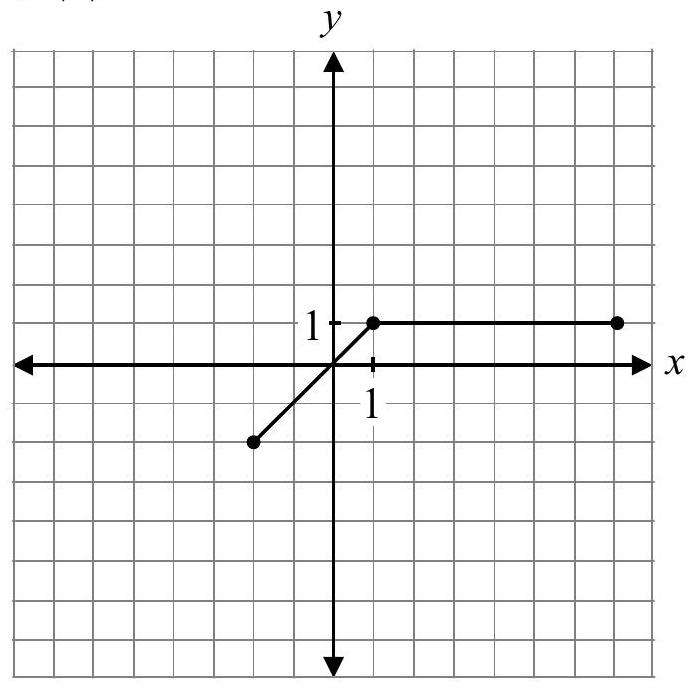
\includegraphics[width=0.6\linewidth]{figures/2795df6c-6e2d-4017-aae1-564aebe344d4-18_688_695_526_298}
\end{center}

\begin{figure}[h]
\begin{center}
\caption{$g(x)$}
  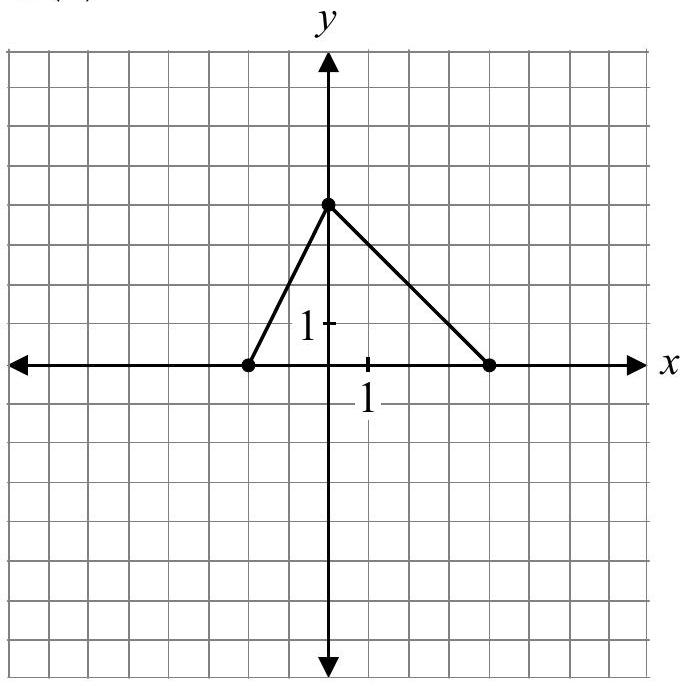
\includegraphics[width=0.6\linewidth]{figures/2795df6c-6e2d-4017-aae1-564aebe344d4-18_686_691_526_1168}
\end{center}
\end{figure}

Sketch the graph of $f(x)+g(x)$.
\begin{solution}
\textbf{Solution:}\par
\begin{center}
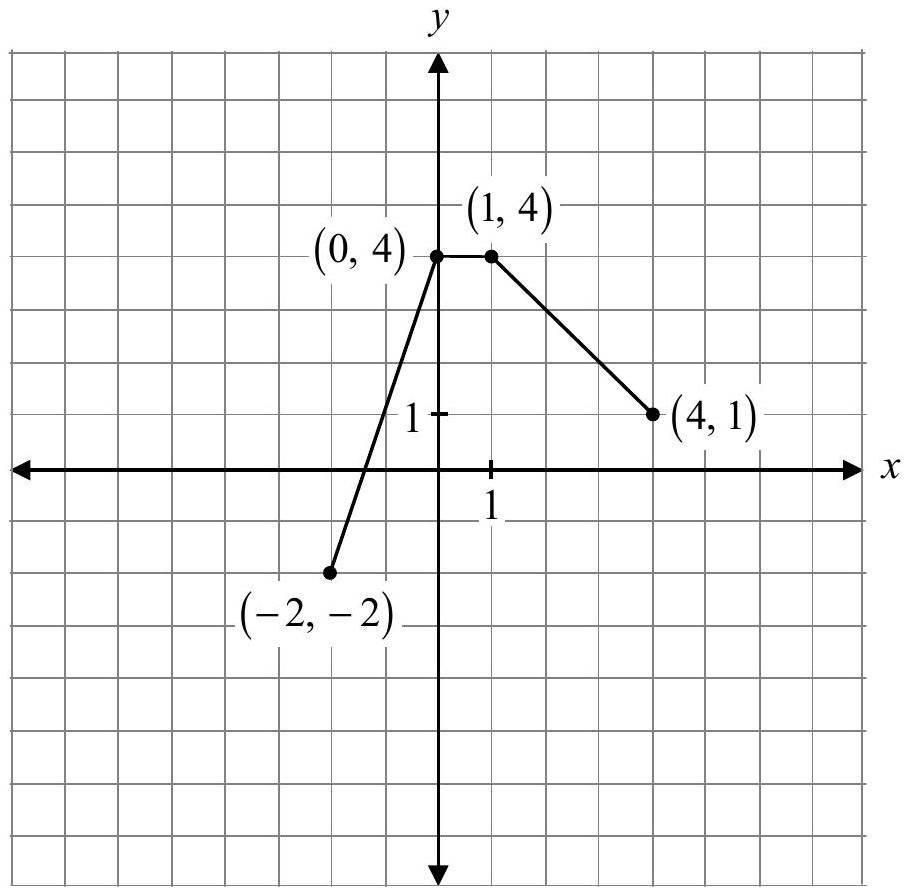
\includegraphics[width=0.6\linewidth]{figures/2795df6c-6e2d-4017-aae1-564aebe344d4-18_894_912_1433_249}
\end{center}

2 marks ( $\frac{1}{2}$ mark for each point where the graph changes direction)

$$
[(-2,-2) ;(0,4) ;(1,4) ;(4,1)]
$$

\begin{center}

\includegraphics[width=0.6\linewidth]{figures/2795df6c-6e2d-4017-aae1-564aebe344d4-18_135_234_1703_1179}
\end{center}

Note(s):

\begin{itemize}
  \item deduct a maximum of 1 mark for incorrect domain
\end{itemize}
\end{solution}

\question
\leavevmode
% Q16 | Pre-Calculus 40S --- January 2013
If $(2,3)$ is a point on the graph of $y=f(x)$, what point must be on the graph of $y=3 f\left(\frac{1}{4} x\right)$ ?\\
\begin{choices}
\choice $\left(\frac{1}{2}, 1\right)$
\choice $\left(\frac{1}{2}, 9\right)$
\choice $(8,1)$
\choice $(8,9)$
\end{choices}
\begin{solution}
\textbf{Solution:}\par
Answers will vary but $b^{3}=a$.\\
Some possible solutions are: $a=8 \quad b=2$\\
or

$$
a=27 \quad b=3
$$

or

$$
a=64 \quad b=4
$$

The range of the graph of $y=f(x)$ is $[-3,2]$.\\
Explain why there is no effect on the range of the graph that is a result of the transformation $y=f(-x)$.

$y=f(-x)$ is a reflection over the $y$-axis.\\
The domain is affected, but the range remains the same.

1 mark for explanation\\
1 mark
\end{solution}

\question
\leavevmode
% Q17 | Pre-Calculus 40S --- January 2013
Sketch the graph of $y=(x+1)(x-2)^{2}(x+5)$.\\
Identify the $x$-intercepts and $y$-intercept.
\begin{solution}
\textbf{Solution:}\par
$x$-intercepts: $-5,-1$, and 2\\
$y$-intercept: 20\\
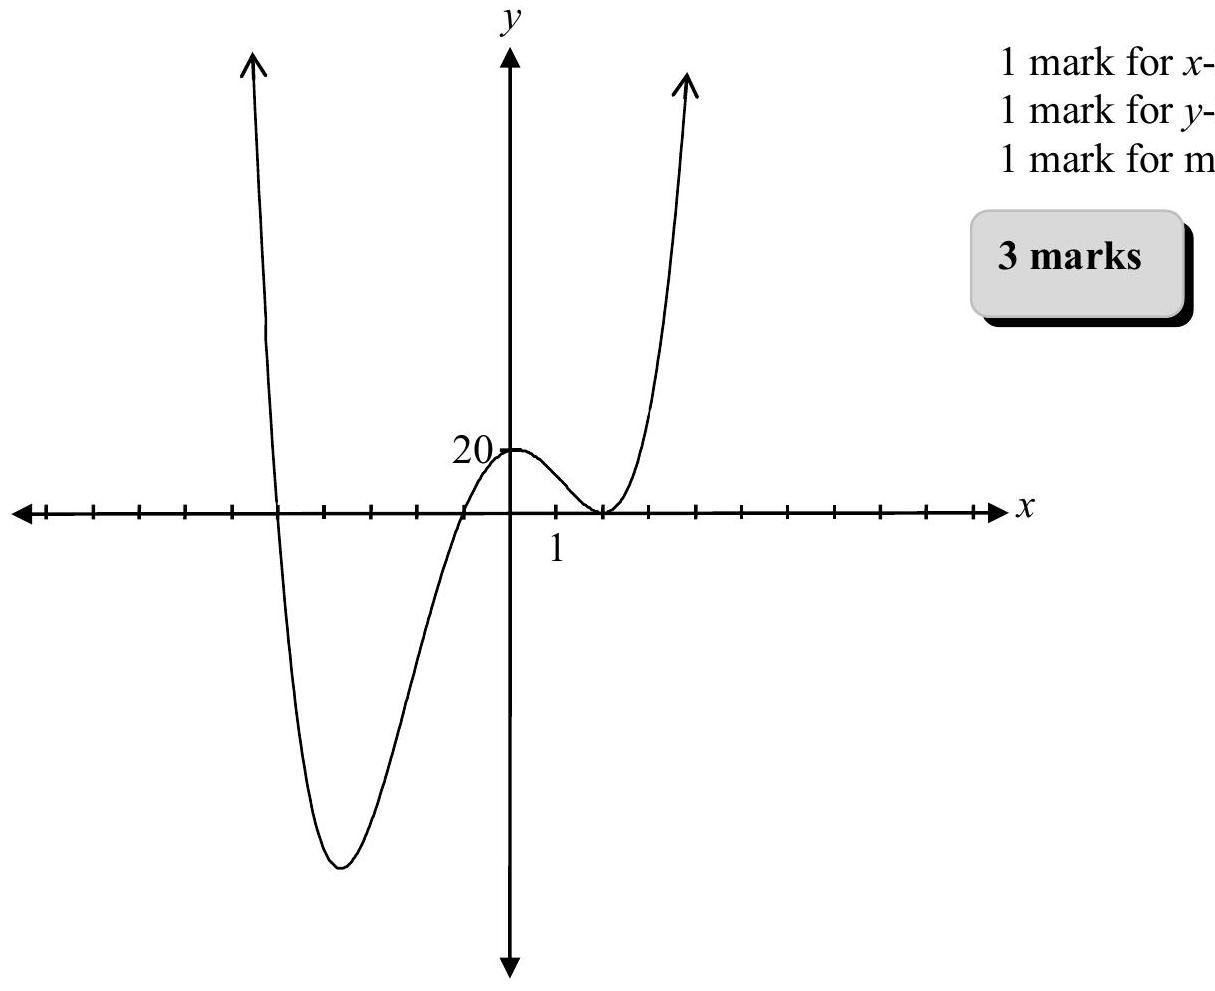
\includegraphics[width=0.6\linewidth]{figures/2795df6c-6e2d-4017-aae1-564aebe344d4-23_991_1215_859_210}

Note(s):

\begin{itemize}
  \item if no graph is shown, give $\frac{1}{2}$ mark for $x$-intercepts $\left(-5,-1\right.$, and 2 ) and $\frac{1}{2}$ mark for $y$-intercept (20)
  \item relative maximum and minimum are not required
\end{itemize}
\end{solution}

\question
\leavevmode
% Q18 | Pre-Calculus 40S --- January 2013
The graph of the function $y=\sin x$ has been transformed to create a new graph.\\
The range of this new graph is $[-4,4]$ and the zeros are $x=k \frac{\pi}{2}$, where $k$ is an integer.\\
Write the equation that corresponds to this new graph.
\begin{solution}
\textbf{Solution:}\par
$$
\begin{aligned}
\text { Amplitude } & =4 & & 1 \text { mark for correct amplitude } \\
\text { Period } & =\pi & & 1 / 2 \text { mark for correct period } \\
\therefore b & =\frac{2 \pi}{\pi}=2 & & 1 / 2 \text { mark for consistent value of } b \\
y & =4 \sin (2 x) & & \mathbf{2} \text { marks }
\end{aligned}
$$

or

Note(s):

\begin{itemize}
  \item deduct $\frac{1}{2}$ mark for a translation that results in an incorrect range and/or zeros
\end{itemize}
\end{solution}

\question
\leavevmode
% Q19 | Pre-Calculus 40S --- January 2013
Given the functions $f(x)=x^{2}-1$ and $g(x)=x+1$, state the domain of $\frac{g(x)}{f(x)}$.
\begin{solution}
\textbf{Solution:}\par
Domain: $x \in \mathbb{R}$ where $x \neq 1$ and $x \neq-1$ 1 mark ( $\frac{1}{2}$ mark for $x \neq 1, \frac{1}{2}$ mark for $x \neq-1$ )\\
a) Sketch the graph of $y=3^{x}$.\\
b) Explain how the graph of $y=3^{x}$ can be used to sketch the graph of $y=\log _{3} x$.

a)\\
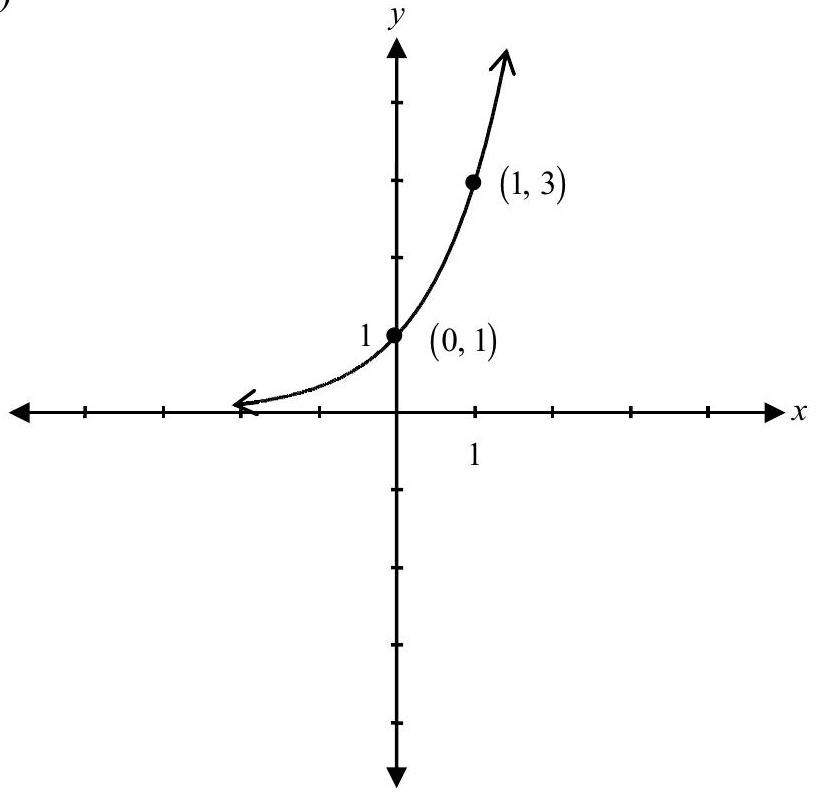
\includegraphics[width=0.6\linewidth]{figures/2795df6c-6e2d-4017-aae1-564aebe344d4-25_796_816_708_214}\\
$\frac{1}{2}$ mark for increasing exponential function\\
$\frac{1}{2}$ mark for $y$-intercept at $(0,1)$\\
$\frac{1}{2}$ mark for consistent point on exponential function\\
$\frac{1}{2}$ mark for asymptotic behaviour\\
2 marks\\
b)

To graph $y=\log _{3} x$, you can reflect the graph of $y=3^{x}$ over the line $y=x$.\\
or\\
You can switch the $x$ and $y$ coordinates of $y=3^{x}$ to get the graph of $y=\log _{3} x$.

1 mark for explanation\\
1 mark

Note(s):

\begin{itemize}
  \item in (b), give $\frac{1}{2}$ mark for having only stated they are inverse functions of each other
\end{itemize}
\end{solution}

\question
\leavevmode
% Q20 | Pre-Calculus 40S --- January 2013
A box in the shape of a rectangular prism has side lengths $x, x+2$, and $x+10$.\\
Write a function, $V(x)$, to express the volume of the box in terms of $x$.\\
Find all possible values of $x$, given that the volume of the box is $96 \mathrm{~cm}^{3}$.\\
State the dimensions of the box.
\begin{solution}
\textbf{Solution:}\par
$$
\begin{array}{rlrl}
V(x) & =(x)(x+2)(x+10) & 1 / 2 \text { mark for expressing volume in terms of } x \\
96 & =(x)(x+2)(x+10) & \\
96 & =x^{3}+12 x^{2}+20 x & \\
0 & =x^{3}+12 x^{2}+20 x-96 & 1 / 2 \text { mark for equating to zero }
\end{array}
$$
\end{solution}

\question
\leavevmode
% Q21 | Pre-Calculus 40S --- January 2013
when $x=2$ :

$$
\begin{aligned}
& 0=(2)^{3}+12(2)^{2}+20(2)-96 \\
& 0=8+48+40-96 \\
& 0=0
\end{aligned}
$$

$\therefore x=2$ is a possible value.\\
1 mark for identifying one possible value of $x$

2 \begin{tabular}{rrrr}
1 & 12 & 20 & -96 \\
 & 2 & 28 & 96 \\
\hline
1 & 14 & 48 & 0 \\
\hline
\end{tabular}

\begin{center}
\begin{tabular}{|l|l|}
\hline
\( \begin{aligned} (x-2)\left(x^{2}+14 x+48\right) & =0 \\ (x-2)(x+8)(x+6) & =0 \\ x & =-8,-6,2 \\ x & \neq-8 \text { and } x \neq-6 \text { because dimensions } \\ & \text { cannot be negative values. } \\ \therefore x & =2 \text { is the only solution. } \end{aligned} \) & 1 mark for division \\
\hline
The dimensions of the box are $2 \mathrm{~cm} \times 4 \mathrm{~cm} \times 12 \mathrm{~cm}$. & $\frac{1}{2}$ mark for stating the dimensions of the box \\
\hline
\end{tabular}
\end{center}

Given the graph of $f(x)$ below, sketch the graph of $y=-f(x)$.\\
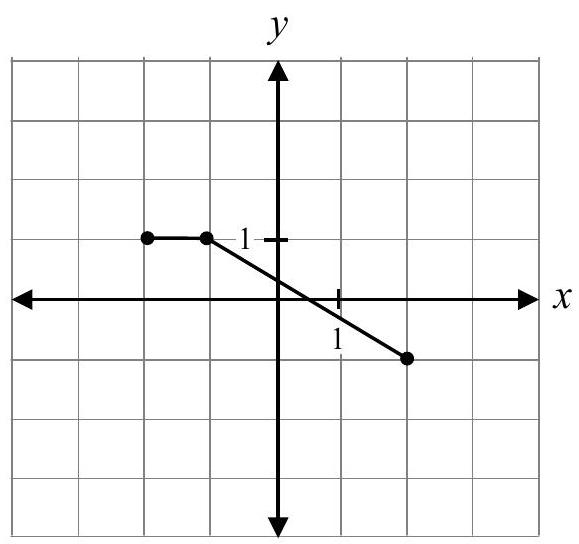
\includegraphics[width=0.6\linewidth]{figures/2795df6c-6e2d-4017-aae1-564aebe344d4-27_544_579_569_259}
\begin{solution}
\textbf{Solution:}\par
\begin{center}
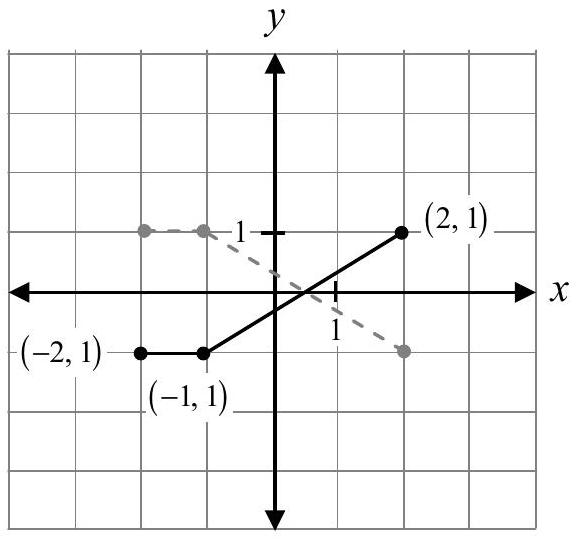
\includegraphics[width=0.6\linewidth]{figures/2795df6c-6e2d-4017-aae1-564aebe344d4-27_540_578_567_1014}
\end{center}

Determine the coordinates of a point $(x, y)$ on the unit circle if you are given $\theta=30^{\circ}$ where $\theta$ is in standard position.

$\mathrm{P}(\theta)=(\cos \theta, \sin \theta)$\\
If $\theta=30^{\circ}$, then the coordinates of $\mathrm{P}(\theta)$ would be $\left(\cos 30^{\circ}, \sin 30^{\circ}\right)$.

1 mark for answer stated as coordinate point\\
or\\
$\mathrm{P}\left(30^{\circ}\right)=\left(\frac{\sqrt{3}}{2}, \frac{1}{2}\right)$

Given the following sinusoidal equation:

$$
P(t)=3000 \sin \left[\frac{\pi}{10}(t-2010)\right]+10000
$$

Determine the maximum value of $\mathrm{P}(t)$ and a value of $t$ at which this maximum occurs.


\textbf{Method 1}\par
$$
\begin{aligned}
\text { Maximum value } & =10000+3000 & & 1 \text { mark for maximum value } \\
& =13000 & & \\
13000 & =3000 \sin \left[\frac{\pi}{10}(t-2010)\right]+10000 & & \\
3000 & =3000 \sin \left[\frac{\pi}{10}(t-2010)\right] & & 1 / 2 \text { mark for simplifying } \\
1 & =\sin \left[\frac{\pi}{10}(t-2010)\right] & & 1 \text { mark for exact value } \\
\frac{\pi}{2} & =\frac{\pi}{10}(t-2010) & & 1 / 2 \text { mark for solving for } t \\
5 & =t-2010 & & \mathbf{3} \text { marks } \\
t & =2015 & &
\end{aligned}
$$

Note(s):

\begin{itemize}
  \item the period of the function is $20 \therefore$ other acceptable answers are: $t=2015 \pm 20$
\end{itemize}


\textbf{Method 2}\par
\begin{center}
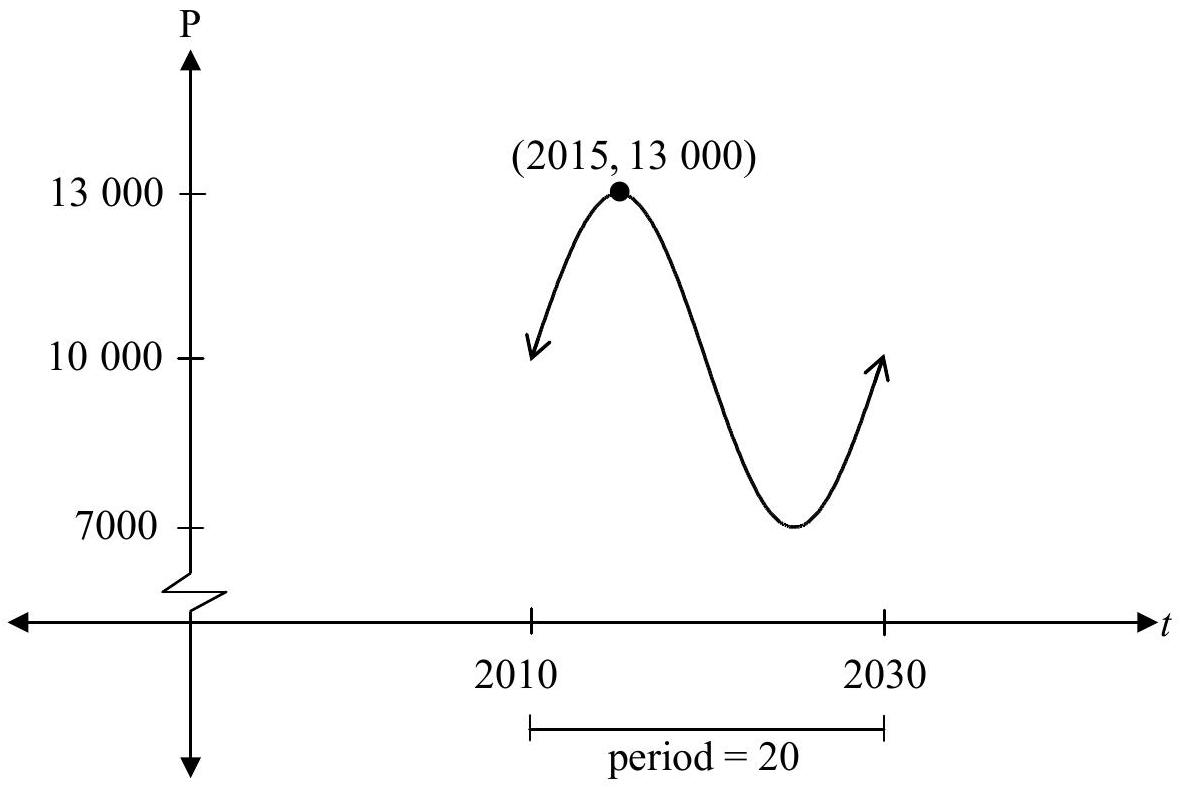
\includegraphics[width=0.6\linewidth]{figures/2795df6c-6e2d-4017-aae1-564aebe344d4-29_787_1180_638_174}
\end{center}

1 mark for period

$$
\begin{aligned}
\mathrm{P}(t) & =13000 \\
t & =2015
\end{aligned}
$$

the maximum value is 13000 when $t=2015$.

1 mark for maximum value\\
1 mark for solving for $t$\\
3 marks
\end{solution}

\question
\leavevmode
% Q22 | Pre-Calculus 40S --- January 2013
Sketch the graph of $y=\sqrt{2 x-2}$.
\begin{solution}
\textbf{Solution:}\par

\textbf{Method 1}\par
$$
\begin{aligned}
y & =\sqrt{2 x-2} \\
& =\sqrt{2(x-1)}
\end{aligned}
$$

\begin{center}
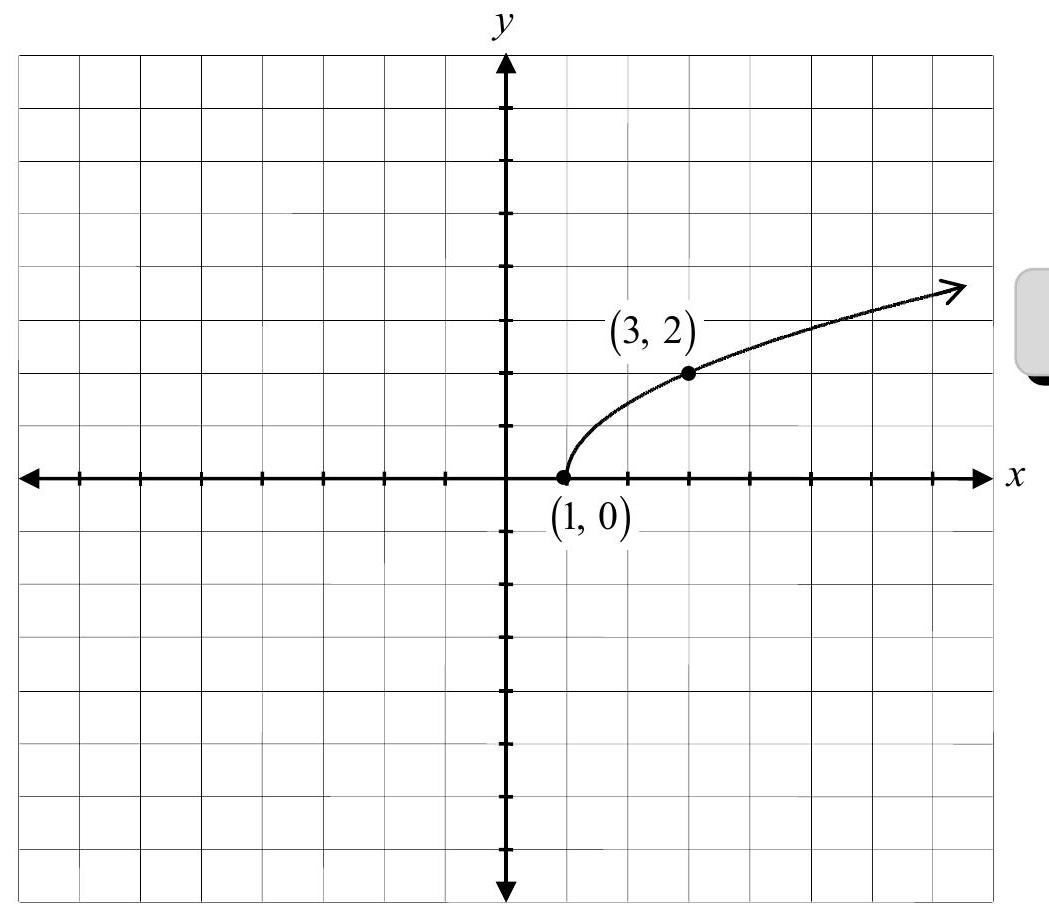
\includegraphics[width=0.6\linewidth]{figures/2795df6c-6e2d-4017-aae1-564aebe344d4-30_922_1049_928_163}
\end{center}

1 mark for domain: $[1, \infty)$\\
1 mark for shape (graph of a radical function)\\
1 mark for horizontal compression\\
3 marks


\textbf{Method 2}\par
\begin{center}
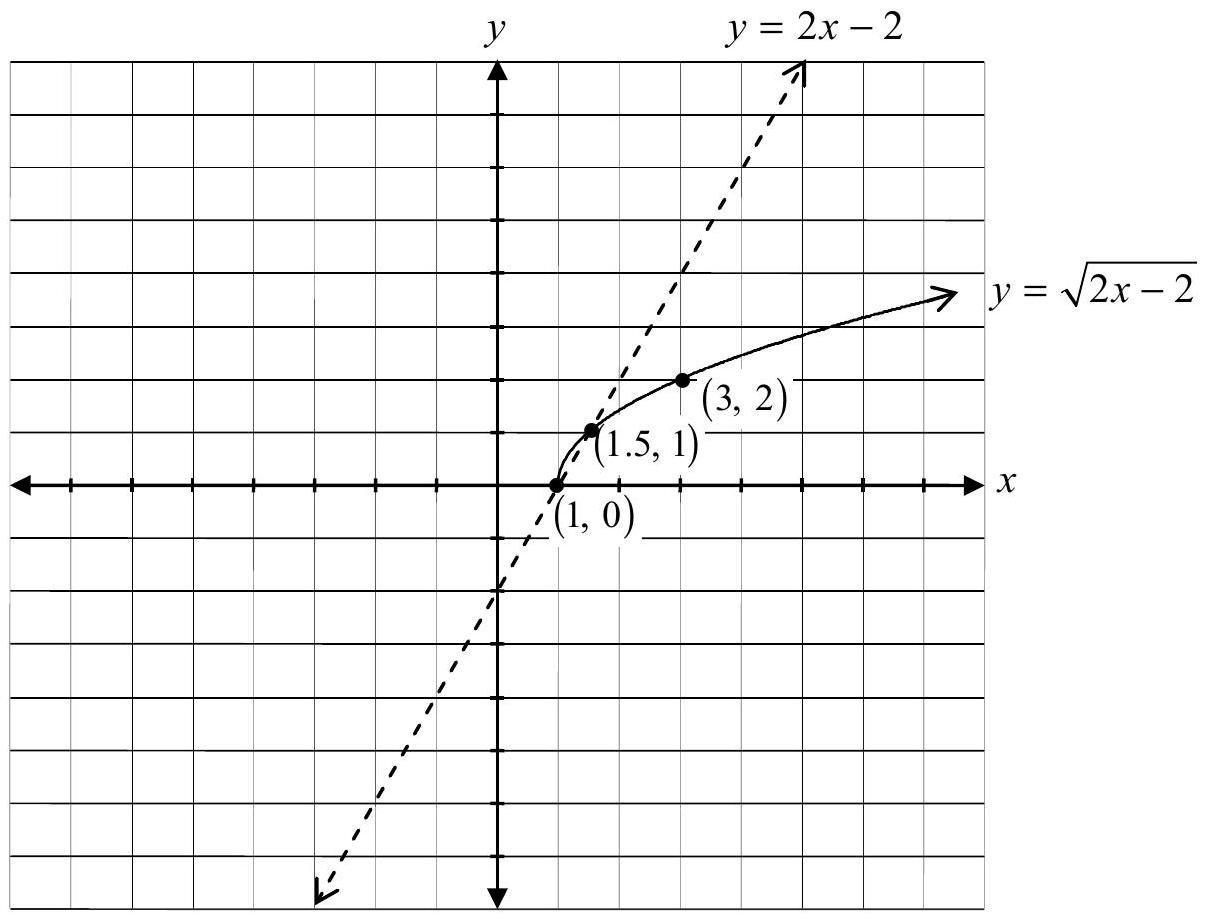
\includegraphics[width=0.6\linewidth]{figures/2795df6c-6e2d-4017-aae1-564aebe344d4-31_921_1209_431_225}
\end{center}

1 mark for domain of $y=\sqrt{2 x-2}:[1, \infty)$\\
1 mark for invariant points where $y=0$ and $y=1$ ( $\frac{1}{2}$ mark for each point)\\
$\frac{1}{2}$ mark for graph of $y=\sqrt{2 x-2}$ drawn above the graph of $y=2 x-2$ between the invariant points $\frac{1}{2}$ mark for graph of $y=\sqrt{2 x-2}$ drawn below the graph of $y=2 x-2$ after the invariant point where $y=1$\\
\\
3 marks
\end{solution}

\question
\leavevmode
% Q23 | Pre-Calculus 40S --- January 2013
Given $f(x)=2 x-6$, write the equation of $f^{-1}(x)$.
\begin{solution}
\textbf{Solution:}\par
Switch the $x$ and $y$ values.

$$
x=2 y-6
$$

1 mark for switching $x$ and $y$ values

$$
\begin{aligned}
& x+6=2 y \\
& \frac{x+6}{2}=y
\end{aligned}
$$

$\frac{1}{2}$ mark for solving for $y$\\
$\therefore f^{-1}(x)=\frac{x+6}{2}$\\
$\frac{1}{2}$ mark for writing equation of $f^{-1}(x)$


\end{solution}

\question
\leavevmode
% Q24 | Pre-Calculus 40S --- January 2013
Question 37\\
R8

Frank tried to expand a logarithmic expression using the laws of logarithms. He made one error.\\
Frank's solution: $\log _{a} \frac{(x+2)}{z w}=\log _{a} x+\log _{a} 2-\log _{a} z-\log _{a} w$\\
Write the correct solution.
\begin{solution}
\textbf{Solution:}\par
Correct solution: $\log _{a} \frac{(x+2)}{z w}=\log _{a}(x+2)-\log _{a} z-\log _{a} w$

1 mark for correct solution\\
1 mark
\end{solution}

\question
\leavevmode
% Q25 | Pre-Calculus 40S --- January 2013
Determine all non-permissible values of $\theta$ over the interval $[0,2 \pi]$.

$$
\frac{\sin \theta}{1+\cos \theta}+\csc \theta+\cot \theta
$$

Explain your reasoning.
\begin{solution}
\textbf{Solution:}\par
To determine non-permissible values, the denominator 1 mark for explanation needs to equal zero.

The denominators of this expression are " $1+\cos \theta$ " and " $\sin \theta$ " (since $\csc \theta=\frac{1}{\sin \theta}$ and $\cot \theta=\frac{\cos \theta}{\sin \theta}$ ).

1 mark ( $\frac{1}{2}$ mark for identifying each restriction)

$$
\begin{aligned}
\therefore 1+\cos \theta & =0 & \sin \theta & =0 \\
\cos \theta & =-1 & \theta & =0, \pi, 2 \pi \\
\theta & =\pi & &
\end{aligned}
$$

1 mark for all non-permissible values of $\theta$ ( $\frac{1}{2}$ mark for each equation)\\
the non-permissible values of $\theta$ over $[0,2 \pi]$ are $0, \pi$, and $2 \pi$.

Given the following graphs:\\
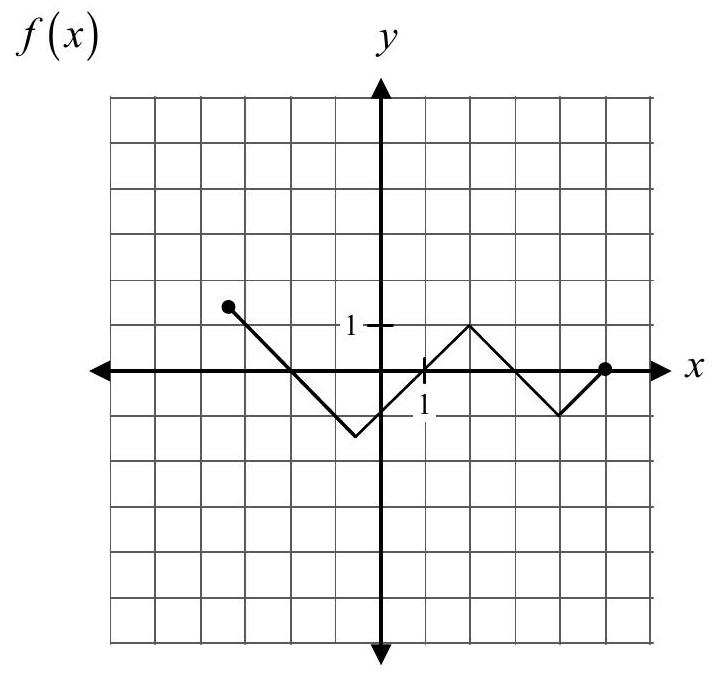
\includegraphics[width=0.6\linewidth]{figures/2795df6c-6e2d-4017-aae1-564aebe344d4-34_678_717_483_283}\\
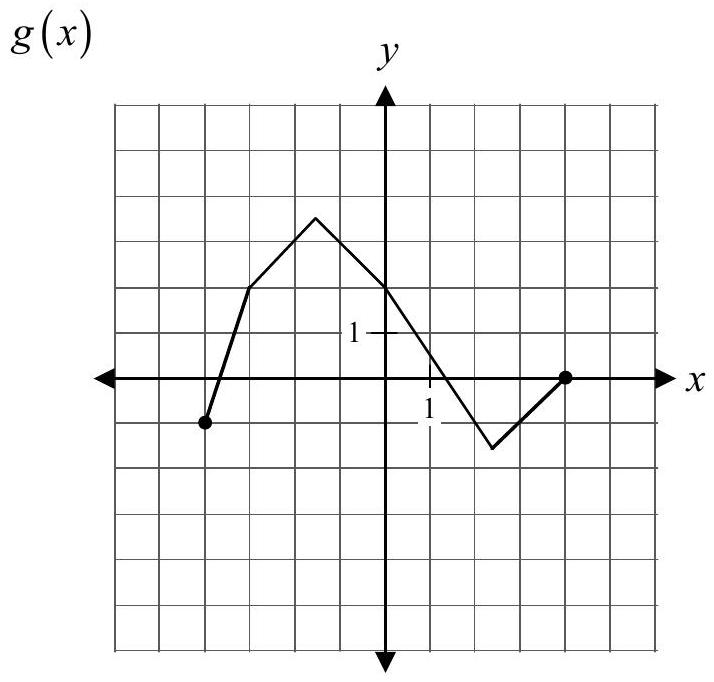
\includegraphics[width=0.6\linewidth]{figures/2795df6c-6e2d-4017-aae1-564aebe344d4-34_682_714_485_1119}\\
a) Determine the value of $[f \cdot g](0)$.\\
b) Determine the value of $g(f(4))$.\\
c) Determine a value for $k$ where $f(k)=1$.

a) $f(0)=-1$

$$
g(0)=2
$$

$$
\begin{aligned}
{[f \cdot g](0) } & =(-1)(2) \\
& =-2
\end{aligned}
$$

b) $f(4)=-1$

$$
g(-1)=3
$$

1 mark for the value of $[f \cdot g](0)$

$\frac{1}{2}$ mark for $f(4)$\\
$\frac{1}{2}$ mark for $g(f(4))$ consistent with $f(4)$ value

1 mark for a value for $k$\\
1 mark
\end{solution}

\question
\leavevmode
% Q26 | Pre-Calculus 40S --- January 2013
Given that $h(x)=2 x^{2}+5 x-3$ and that $h(x)=f(x) \cdot g(x)$, determine $f(x)$ and $g(x)$.
\begin{solution}
\textbf{Solution:}\par
$$
\begin{aligned}
& f(x)=2 x-1 \\
& g(x)=x+3
\end{aligned}
$$

1 mark for two correct factors of $h(x)$\\
1 mark\\
Other answers are possible.\\
Question 41

The graph of $y=2 \cos \theta+1$ below can be used to solve the equation $\cos \theta=-\frac{1}{2}$ over the interval $[-2 \pi, 2 \pi]$. Indicate on the graph where to find the solutions to the equation $\cos \theta=-\frac{1}{2}$.

The solution to the equation $\cos \theta=-\frac{1}{2}$ is found where the graph of $y=2 \cos \theta+1$ crosses the $x$-axis.\\
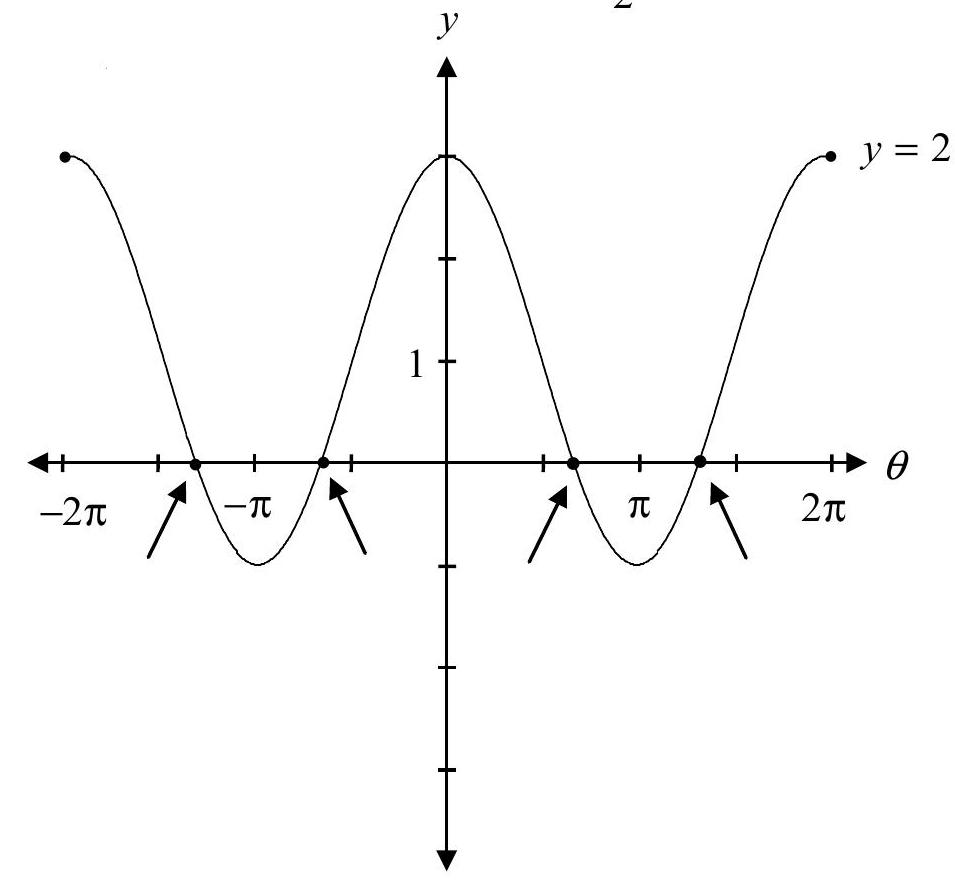
\includegraphics[width=0.6\linewidth]{figures/2795df6c-6e2d-4017-aae1-564aebe344d4-35_884_955_1499_229}

1 mark for indicating solutions on graph 1 mark

Note(s):

\begin{itemize}
  \item give $\frac{1}{2}$ mark for indicating 1,2 , or 3 of the solutions
\end{itemize}
\end{solution}

\question
\leavevmode
% Q27 | Pre-Calculus 40S --- January 2013
The function $f(x)$ is transformed.\\
A new function, $y=\frac{1}{f(x)}$, is created that does not have any vertical asymptotes.\\
What can you conclude about the original function $f(x)$ ?
\begin{solution}
\textbf{Solution:}\par
If $f(x)$ does not have any $x$-intercepts, then the transformation would not have any vertical asymptotes.\\
or\\
$f(x)$ cannot equal zero.\\
or

$$
f \neq 0
$$

1 mark for conclusion\\
1 mark

Note(s):

\begin{itemize}
  \item award $\frac{1}{2}$ mark for a correct example without a given conclusion
\end{itemize}
\end{solution}

\question
\leavevmode
% Q28 | Pre-Calculus 40S --- January 2013
Draw the angle $-\frac{7 \pi}{8}$ in standard position.
\begin{solution}
\textbf{Solution:}\par
\begin{center}
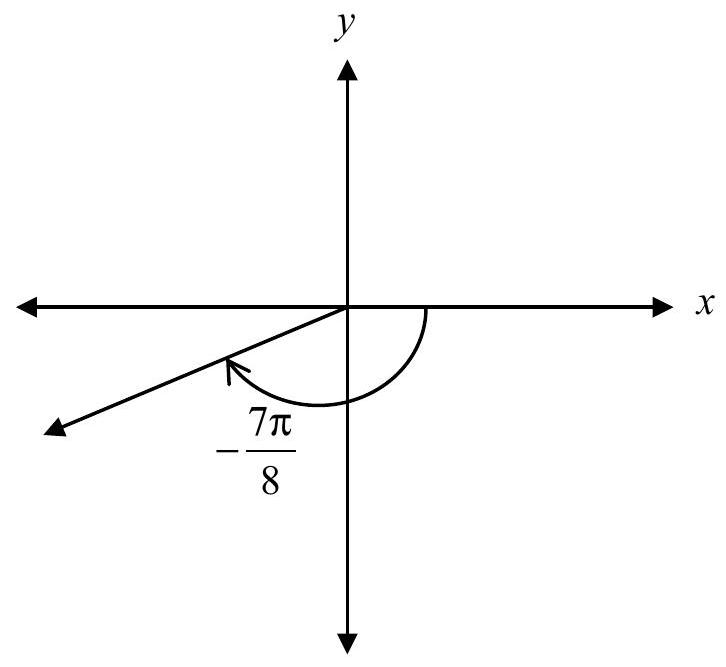
\includegraphics[width=0.6\linewidth]{figures/2795df6c-6e2d-4017-aae1-564aebe344d4-36_667_726_1935_216}
\end{center}

1 mark for angle drawn in Quadrant III\\
1 mark
\end{solution}

\question
\leavevmode
% Q29 | Pre-Calculus 40S --- January 2013
Determine the exact value of:

$$
4 \cos \left(\frac{11 \pi}{12}\right)
$$
\begin{solution}
\textbf{Solution:}\par

\textbf{Method 1}\par
$$
\begin{array}{rlr}
4 \cos \left(\frac{11 \pi}{12}\right) & =4 \cos \left(\frac{\pi}{4}+\frac{2 \pi}{3}\right) & 1 \text { mark for combination } \\
& =4\left[\cos \frac{\pi}{4} \cos \frac{2 \pi}{3}-\sin \frac{\pi}{4} \sin \frac{2 \pi}{3}\right] & \\
& =4\left[\left(\frac{\sqrt{2}}{2}\right)\left(-\frac{1}{2}\right)-\left(\frac{\sqrt{2}}{2}\right)\left(\frac{\sqrt{3}}{2}\right)\right] & 2 \text { marks }\left(\frac{1}{2} \text { mark for each exact value }\right) \\
& =4\left[\frac{-\sqrt{2}-\sqrt{6}}{4}\right] & 3 \text { marks } \\
& =-\sqrt{2}-\sqrt{6}
\end{array}
$$


\textbf{Method 2}\par
$\frac{11 \pi}{12}$ has a reference angle of $\frac{\pi}{12}$.

$$
\begin{aligned}
\cos \left(\frac{\pi}{12}\right) & =\cos \left(\frac{\pi}{4}-\frac{\pi}{6}\right) \\
& =\cos \frac{\pi}{4} \cos \frac{\pi}{6}+\sin \frac{\pi}{4} \sin \frac{\pi}{6} \\
& =\left(\frac{\sqrt{2}}{2}\right)\left(\frac{\sqrt{3}}{2}\right)+\left(\frac{\sqrt{2}}{2}\right)\left(\frac{1}{2}\right) \\
& =\frac{\sqrt{6}+\sqrt{2}}{4}
\end{aligned}
$$

Since $\frac{11 \pi}{12}$ is in Quadrant II, cosine is negative.\\
$\therefore 4 \cos \left(\frac{11 \pi}{12}\right)=4\left(\frac{-\sqrt{6}-\sqrt{2}}{4}\right)$

$$
=-\sqrt{6}-\sqrt{2}
$$

$\frac{1}{2}$ mark for correct reference angle\\
$\frac{1}{2}$ mark for substitution into correct identity

1 mark for exact values

1 mark for the concept that $\cos \left(\frac{11 \pi}{12}\right)$ is $<0$

Note(s):

\begin{itemize}
  \item $\frac{-2-2 \sqrt{3}}{\sqrt{2}}$ is an acceptable way to write the solution
  \item in Method 1 , another possible combination is $\left(\frac{\pi}{6}+\frac{3 \pi}{4}\right)$
  \item deduct $\frac{1}{2}$ mark if answer is not expressed as a single fraction
  \item in Method 2, the reference angle need not be explicitly stated in order to obtain full marks
\end{itemize}
\end{solution}

\question
\leavevmode
% Q30 | Pre-Calculus 40S --- January 2013
Sketch the graph of $f(x)=\frac{x-4}{x^{2}-3 x-4}$.
\begin{solution}
\textbf{Solution:}\par
\begin{center}
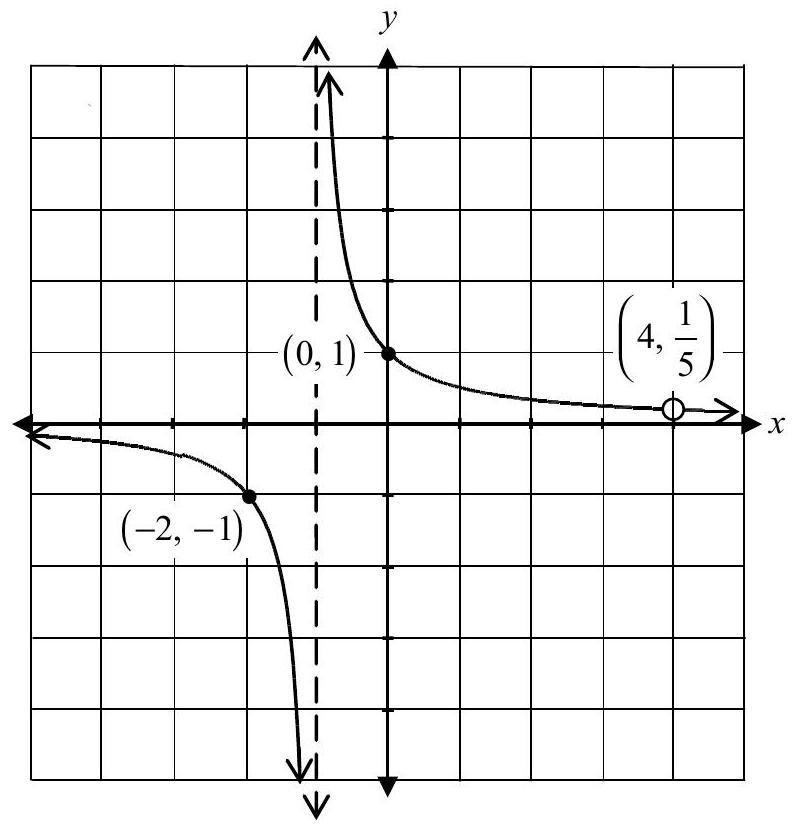
\includegraphics[width=0.6\linewidth]{figures/2795df6c-6e2d-4017-aae1-564aebe344d4-39_829_796_708_212}
\end{center}

1 mark for vertical asymptote at $x=-1$\\
$\frac{1}{2}$ mark for graph left of vertical asymptote\\
$\frac{1}{2}$ mark for graph right of vertical asymptote 1 mark for point of discontinuity at $x=4$

3 marks
\end{solution}

\question
\leavevmode
% Q31 | Pre-Calculus 40S --- January 2013
$$
\begin{aligned}
f(x) & =\frac{x-4}{x^{2}-3 x-4} \\
& =\frac{x-4}{(x-4)(x+1)} \\
& =\frac{1}{x+1} \text { with a point of discontinuity at } x=4
\end{aligned}
$$

point of discontinuity: $f(4)=\frac{1}{5}$\\
there is a point of discontinuity at $\left(4, \frac{1}{5}\right)$

$$
y \text {-intercept: } \begin{aligned}
f(0) & =\frac{0-4}{(0)^{2}-3(0)-4} \\
& =\frac{-4}{-4} \\
& =1
\end{aligned}
$$

Estimate the value of $\log _{5} 35$.\\
Justify your answer.
\begin{solution}
\textbf{Solution:}\par
$$
5^{2}=25 \quad 5^{3}=125
$$

The value of $\log _{5} 35$ is more than 2 but less than 2.5.

$$
\frac{1}{2} \text { mark for justification }
$$

$\frac{1}{2}$ mark for estimated answer


\end{solution}

\question
\leavevmode
% Q32 | Pre-Calculus 40S --- January 2013
If $p(x)=x^{5}-12 x+1$, determine the remainder when $p(x)$ is divided by $(x+2)$.
\begin{solution}
\textbf{Solution:}\par

\textbf{Method 1}\par
$$
\begin{aligned}
p(x) & =x^{5}-12 x+1 \\
p(-2) & =(-2)^{5}-12(-2)+1 \\
& =-32+24+1 \\
& =-7
\end{aligned}
$$


\textbf{Method 2}\par
1 mark for substitution

1 mark

$$
- 2 \div { 1 0 0 0 0 0 0 }
$$

1 mark for correct set-up of synthetic division\\
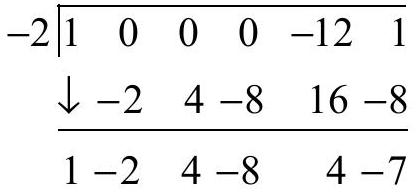
\includegraphics[width=0.6\linewidth]{figures/2795df6c-6e2d-4017-aae1-564aebe344d4-40_195_418_1963_1138}

1 mark
\end{solution}

\question
\leavevmode
% Q33 | Pre-Calculus 40S --- January 2013
The remainder is -7 .

Describe the effects on the graph of $y=f(x)$ when asked for the graph of $y=f(x-3)+5$.
\begin{solution}
\textbf{Solution:}\par
Shift right 3 and up $5 \frac{1}{2}$ mark for horizontal translation\\
$\frac{1}{2}$ mark for vertical translation\\
or\\
1 mark\\
$(x+3, y+5)$

Find the exact value of the following expression:

$$
\sin \left(\frac{11 \pi}{3}\right) \cdot \sec \left(\frac{4 \pi}{3}\right) \cdot \tan \left(-\frac{5 \pi}{6}\right)
$$

$=\left(-\frac{\sqrt{3}}{2}\right)(-2)\left(\frac{1}{\sqrt{3}}\right)$\\
1 mark for $\sin \left(\frac{11 \pi}{3}\right)\left(\frac{1}{2}\right.$ mark for quadrant, $\frac{1}{2}$ mark for value $)$\\
$=1$\\
1 mark for $\sec \left(\frac{4 \pi}{3}\right)\left(\frac{1}{2}\right.$ mark for quadrant, $1 / 2$ mark for value)\\
1 mark for $\tan \left(-\frac{5 \pi}{6}\right)\left(\frac{1}{2}\right.$ mark for quadrant, $1 / 2$ mark for value $)$\\
3 marks
\end{solution}

\end{questions}
\end{document}
